\chapter{突变与基因组多样化}\label{ch:b2:genome-diversification}

在加有抗生素的平板上涂布十亿个细菌，
次日清晨便长出了几个菌落。这种药物
是否教会了这些细胞抵抗它，还是它们在接触药物之前就已具有抗性？
这个问题听起来颇具哲学意味，并已在
1943 年由一项设计极为精巧的实验解决：抗性
细胞早已存在，由\omterm{def:b2:genome-diversification:mutation}{突变}产生，这些\omterm{def:b2:genome-diversification:mutation}{突变}
随机发生，与其是否有用无关。本章讨论这些变异的
来源——复制错误、化学
意外、跳跃基因、细胞间传递的基因、
基因及整个基因组的重复——以及这些变异的
发生速率。选择负责筛选这些变异，其内容见
\cref{ch:b2:population-genetics}；本章讨论的是原材料
从何而来。

\section{突变}

\begin{definition}[突变及其类型]\label{def:b2:genome-diversification:mutation}
\index{突变}\index{点突变}\index{移码}\index{染色体重排}
\emph{突变}是基因组序列中可遗传的
改变。\emph{点突变}只改变一个或几个碱基：
\emph{替换}用一个碱基取代另一个碱基（
\emph{转换}是指嘌呤与嘌呤、嘧啶与嘧啶之间的互换，
即 A$\leftrightarrow$G 或 C$\leftrightarrow$T；
\emph{颠换}则在两类之间互换）；\emph{插入}或
\emph{缺失}会增加或删除碱基。在编码序列中，
若替换使新密码子编码的氨基酸不变，则为\emph{沉默突变}；
若编码另一种氨基酸，则为\emph{错义}；若
产生终止，则为\emph{无义}。插入或缺失的碱基数若非三的倍数，
会使阅读框移位（\emph{移码}），使下游
每个密码子都被扰乱。\emph{染色体重排}会移动大片段：
缺失、重复、倒位，以及染色体之间的
易位。\emph{基因组突变}会改变染色体的
数目：\emph{非整倍性}（比正常数目多或少一条染色体，
如 21 三体）以及\emph{\omterm{def:b2:genome-diversification:polyploidy}{多倍性}}（整套染色体的增加）。
体细胞中的突变只遗传给该细胞的
后代；种系中的突变则遗传给生物体的
后代，而只有这类突变才与演化有关。
\end{definition}

\begin{omfigure}
\begin{tikzpicture}[every node/.style={font=\small\ttfamily}]
  \node[anchor=west] at (0,2.4) {ATG GAA TTC CTG AAG TGG TAA};
  \node[anchor=west, font=\scriptsize\rmfamily] at (5.6,2.4) {Met Glu Phe Leu Lys Trp 终止——野生型};
  \node[anchor=west] at (0,1.7) {ATG GA\textcolor{omThm}{G} TTC CTG AAG TGG TAA};
  \node[anchor=west, font=\scriptsize\rmfamily] at (5.6,1.7) {Met Glu Phe Leu Lys Trp 终止——沉默突变};
  \node[anchor=west] at (0,1.0) {ATG G\textcolor{omThm}{T}A TTC CTG AAG TGG TAA};
  \node[anchor=west, font=\scriptsize\rmfamily] at (5.6,1.0) {Met \textcolor{omThm}{Val} Phe Leu Lys Trp 终止——错义};
  \node[anchor=west] at (0,0.3) {ATG \textcolor{omThm}{T}AA TTC CTG AAG TGG TAA};
  \node[anchor=west, font=\scriptsize\rmfamily] at (5.6,0.3) {Met \textcolor{omThm}{终止}——无义};
  \node[anchor=west] at (0,-0.4) {ATG GA\textcolor{omThm}{C}A TTC CTG AAG TGG TAA};
  \node[anchor=west, font=\scriptsize\rmfamily] at (5.6,-0.4) {Met \textcolor{omThm}{Asp Ile Pro Glu Val} \dots{}——移码};
\end{tikzpicture}

{\small 短编码序列中的\omterm{def:b2:genome-diversification:mutation}{点突变}（改变处以红色标出）。
沉默\omterm{def:b2:genome-diversification:mutation}{突变}不改变蛋白质；错义改变一个
残基；无义使蛋白质截短；单个插入的碱基使
阅读框移位，并改写其下游的全部序列。}
\end{omfigure}

\begin{proposition}[突变的来源]\label{prop:b2:genome-diversification:sources}
\index{诱变剂}\index{脱氨基}\index{脱嘌呤}
三类来源。\emph{复制错误}：DNA 聚合酶错放一个碱基
的频率约为每 $10^{5}$ 个碱基一次；其校对外切核酸酶去除
了大部分错误，余下约每 $10^{7}$ 个碱基一个；错配修复
紧随复制叉进行，以旧链为模板校正新链，使最终
错误率约降至 $10^{-9}$ 至 $10^{-10}$，即每个碱基每次复制。
\emph{自发化学损伤}：每天，每个人体细胞中
约有 \num{10000} 个嘌呤从其脱氧核糖上脱落
（\emph{\omterm{prop:b2:genome-diversification:sources}{脱嘌呤}}），另有一百个胞嘧啶失去氨基
（\emph{\omterm{prop:b2:genome-diversification:sources}{脱氨基}}，使 C 转变为 U，U 与 A 配对）；两者通常都会被修复，
但修复并非总能成功。\emph{\omterm{prop:b2:genome-diversification:sources}{诱变剂}}：紫外线使相邻胸腺嘧啶
形成二聚体；电离辐射使链断裂；
烷基化试剂和亚硝酸改变碱基；嵌入型染料
滑入碱基对之间并引起\omterm{def:b2:genome-diversification:mutation}{移码}；呼吸产生的氧自由基
使鸟嘌呤氧化。每个碱基的\omterm{thm:b2:genome-diversification:rate}{突变速率}很小；将其
乘以基因组大小与细胞数目之后，就不小了。
\end{proposition}

\begin{theorem}[每个基因组与每个种群的突变数]\label{thm:b2:genome-diversification:rate}
\index{突变速率}
若\omterm{thm:b2:genome-diversification:rate}{突变速率}为每个碱基对每次复制 $u$，且
基因组含 $G$ 个碱基对，则每次复制平均产生
$U = uG$ 个新\omterm{def:b2:genome-diversification:mutation}{突变}，由 $N$ 个细胞组成的群体每代产生 $UN$
个\omterm{def:b2:genome-diversification:mutation}{突变}。对于 \emph{E.~coli}（$u \approx \qty{5e-10}{}$，$G =
\qty{4.6e6}{}$）：$U \approx 0.002$，因此每五百个细胞中约有一个
携带新\omterm{def:b2:genome-diversification:mutation}{突变}——但 $10^{9}$ 个细胞的培养物每代产生两
百万个新\omterm{def:b2:genome-diversification:mutation}{突变}，且 $3G \approx 1.4\times
10^{7}$ 种可能的单碱基改变中的每一种都会在其中某处出现，每隔
几代出现一次。对于人类（$u \approx \qty{1.2e-8}{}$，每
代，单倍体组 $G = \qty{3.2e9}{}$，共两组）：每个
孩子平均携带约 \num{75} 个新\omterm{def:b2:genome-diversification:mutation}{突变}，其中一个或两个位于
编码序列中。
\end{theorem}
\begin{proof}
每个碱基在复制时独立地以概率 $u$ 出错，因此
每份基因组拷贝的错误数是 $G$ 个独立
稀有事件之和，均值为 $uG$（近似服从泊松分布）。
$N$ 个细胞产生 $N$ 份拷贝。人类的数值中，$u$ 乘以 $2G$
以计入二倍体基因组；每代速率是按代计的，
而非按复制计，因为生殖细胞在受精与下一次受精
之间要经历许多次复制。
\end{proof}

\begin{theorem}[生长培养物中的突变体]\label{thm:b2:genome-diversification:luria}
\index{卢里亚–德尔布吕克实验}\index{波动试验}
由 $N_0$ 增长到 $N$ 个细胞的培养物中，若某一\omterm{def:b2:genome-diversification:mutation}{突变}
在每次细胞分裂时以概率 $m$ 发生，则培养结束时平均有
$m(N - N_0)$ 次\omterm{def:b2:genome-diversification:mutation}{突变}\emph{事件}，平均的
\emph{\omterm{def:b2:genome-diversification:mutation}{突变}细胞}数为
\[
\langle M\rangle = m\,N\,\ln\frac{N}{N_0},
\]
这一数目大于事件数，因为早期\omterm{def:b2:genome-diversification:mutation}{突变}会奠定一个
克隆。\omterm{def:b2:genome-diversification:mutation}{突变}细胞数在不同培养物之间差异极大
（罕见的早期事件会产生“大奖”），而若\omterm{def:b2:genome-diversification:mutation}{突变}
是在铺板时诱导的，则将服从泊松分布，
方差与均值相等。没有\omterm{def:b2:genome-diversification:mutation}{突变}体的培养物所占比例
为 $p_0 = e^{-m(N - N_0)}$，由此可直接得出 $m$。
\end{theorem}
\begin{proof}
由 $n$ 增长到 $n + \mathrm{d}n$ 个细胞需经历 $\mathrm{d}n$
次分裂，每次分裂都是一次\omterm{def:b2:genome-diversification:mutation}{突变}机会，故 $m\,\mathrm{d}n$
个事件发生于该区间；求和可得总共 $m(N - N_0)$ 个事件。
培养物中有 $n$ 个细胞时发生的\omterm{def:b2:genome-diversification:mutation}{突变}会建立一个
克隆，该克隆与培养物同步生长，结束时共有 $N/n$ 个细胞，
故\omterm{def:b2:genome-diversification:mutation}{突变}细胞的期望数为
$\int_{N_0}^{N} m\,(N/n)\,\mathrm{d}n = mN\ln(N/N_0)$。事件
稀少且相互独立，故其个数服从均值为
$m(N - N_0)$ 的泊松分布，无\omterm{def:b2:genome-diversification:mutation}{突变}的概率为 $e^{-m(N - N_0)}$。
\end{proof}
\begin{proof}[证据]
卢里亚和德尔布吕克（1943 年）培养了二十份小规模的
\emph{E.~coli} 培养物，每份仅由少数几个细胞开始，同时从
一个大培养物中取了二十份样本；将这四十份全部铺板，并加入
一种可杀死所有敏感细胞的噬菌体，并计数了
抗性菌落。来自单一培养物的样本，其计数
接近其均值，正如泊松分布所预言的；而独立培养物的
计数为 0、0、1、0、3、0、107、0、5\dots{}——方差
是均值的许多倍。抗性\omterm{def:b2:genome-diversification:mutation}{突变}在随机的时刻发生，
并且是在细胞接触噬菌体\emph{之前}发生的，早期的\omterm{def:b2:genome-diversification:mutation}{突变}
产生了“大奖”。莱德伯格夫妇（1952 年）证实了这一点，
但从未让被选中的细胞接触该试剂：先将一块绒布
垫在平板上，再盖印出副本，发现抗性
菌落在每个副本的相同位置出现，并将其
从未经处理的母平板上分离出来。
\end{proof}

\begin{omfigure}
\begin{tikzpicture}[every node/.style={font=\scriptsize}, level distance=0.55cm, sibling distance=0.5cm, edge from parent/.style={draw, gray}]
  \begin{scope}
    \node[circle, fill=omDef!40, inner sep=1.5pt] (r) at (0,0) {}
      child { node[circle, fill=omDef!40, inner sep=1.5pt] {}
        child { node[circle, fill=omDef!40, inner sep=1.5pt] {} child { node[circle, fill=omDef!40, inner sep=1.5pt] {} } child { node[circle, fill=omDef!40, inner sep=1.5pt] {} } }
        child { node[circle, fill=omDef!40, inner sep=1.5pt] {} child { node[circle, fill=omDef!40, inner sep=1.5pt] {} } child { node[circle, fill=omThm, inner sep=1.5pt] {} } } }
      child { node[circle, fill=omDef!40, inner sep=1.5pt] {}
        child { node[circle, fill=omDef!40, inner sep=1.5pt] {} child { node[circle, fill=omDef!40, inner sep=1.5pt] {} } child { node[circle, fill=omDef!40, inner sep=1.5pt] {} } }
        child { node[circle, fill=omDef!40, inner sep=1.5pt] {} child { node[circle, fill=omDef!40, inner sep=1.5pt] {} } child { node[circle, fill=omDef!40, inner sep=1.5pt] {} } } };
    \node[align=center] at (0,-2.4) {晚期突变：\\一个突变细胞};
  \end{scope}
  \begin{scope}[xshift=5cm]
    \node[circle, fill=omDef!40, inner sep=1.5pt] at (0,0) {}
      child { node[circle, fill=omThm, inner sep=1.5pt] {}
        child { node[circle, fill=omThm, inner sep=1.5pt] {} child { node[circle, fill=omThm, inner sep=1.5pt] {} } child { node[circle, fill=omThm, inner sep=1.5pt] {} } }
        child { node[circle, fill=omThm, inner sep=1.5pt] {} child { node[circle, fill=omThm, inner sep=1.5pt] {} } child { node[circle, fill=omThm, inner sep=1.5pt] {} } } }
      child { node[circle, fill=omDef!40, inner sep=1.5pt] {}
        child { node[circle, fill=omDef!40, inner sep=1.5pt] {} child { node[circle, fill=omDef!40, inner sep=1.5pt] {} } child { node[circle, fill=omDef!40, inner sep=1.5pt] {} } }
        child { node[circle, fill=omDef!40, inner sep=1.5pt] {} child { node[circle, fill=omDef!40, inner sep=1.5pt] {} } child { node[circle, fill=omDef!40, inner sep=1.5pt] {} } } };
    \node[align=center] at (0,-2.4) {早期突变：\\一次“大奖”，四个突变细胞};
  \end{scope}
  \begin{scope}[xshift=10cm]
    \node[circle, fill=omDef!40, inner sep=1.5pt] at (0,0) {}
      child { node[circle, fill=omDef!40, inner sep=1.5pt] {}
        child { node[circle, fill=omDef!40, inner sep=1.5pt] {} child { node[circle, fill=omDef!40, inner sep=1.5pt] {} } child { node[circle, fill=omThm, inner sep=1.5pt] {} } }
        child { node[circle, fill=omDef!40, inner sep=1.5pt] {} child { node[circle, fill=omDef!40, inner sep=1.5pt] {} } child { node[circle, fill=omDef!40, inner sep=1.5pt] {} } } }
      child { node[circle, fill=omDef!40, inner sep=1.5pt] {}
        child { node[circle, fill=omDef!40, inner sep=1.5pt] {} child { node[circle, fill=omThm, inner sep=1.5pt] {} } child { node[circle, fill=omDef!40, inner sep=1.5pt] {} } }
        child { node[circle, fill=omDef!40, inner sep=1.5pt] {} child { node[circle, fill=omDef!40, inner sep=1.5pt] {} } child { node[circle, fill=omDef!40, inner sep=1.5pt] {} } } };
    \node[align=center] at (0,-2.4) {若在涂布时诱导：\\泊松散布};
  \end{scope}
\end{tikzpicture}

{\small \omterm{thm:b2:genome-diversification:luria}{波动试验}。若\omterm{def:b2:genome-diversification:mutation}{突变}（红色）在生长过程中随机发生，
\omterm{def:b2:genome-diversification:mutation}{突变}体的数目取决于\omterm{def:b2:genome-diversification:mutation}{突变}\emph{何时}发生，
独立培养物之间差异极大；若选择剂是在涂布时诱导\omterm{def:b2:genome-diversification:mutation}{突变}的，
每个培养物都会显示
出相近的较小数目。}
\end{omfigure}

\begin{omfigure}
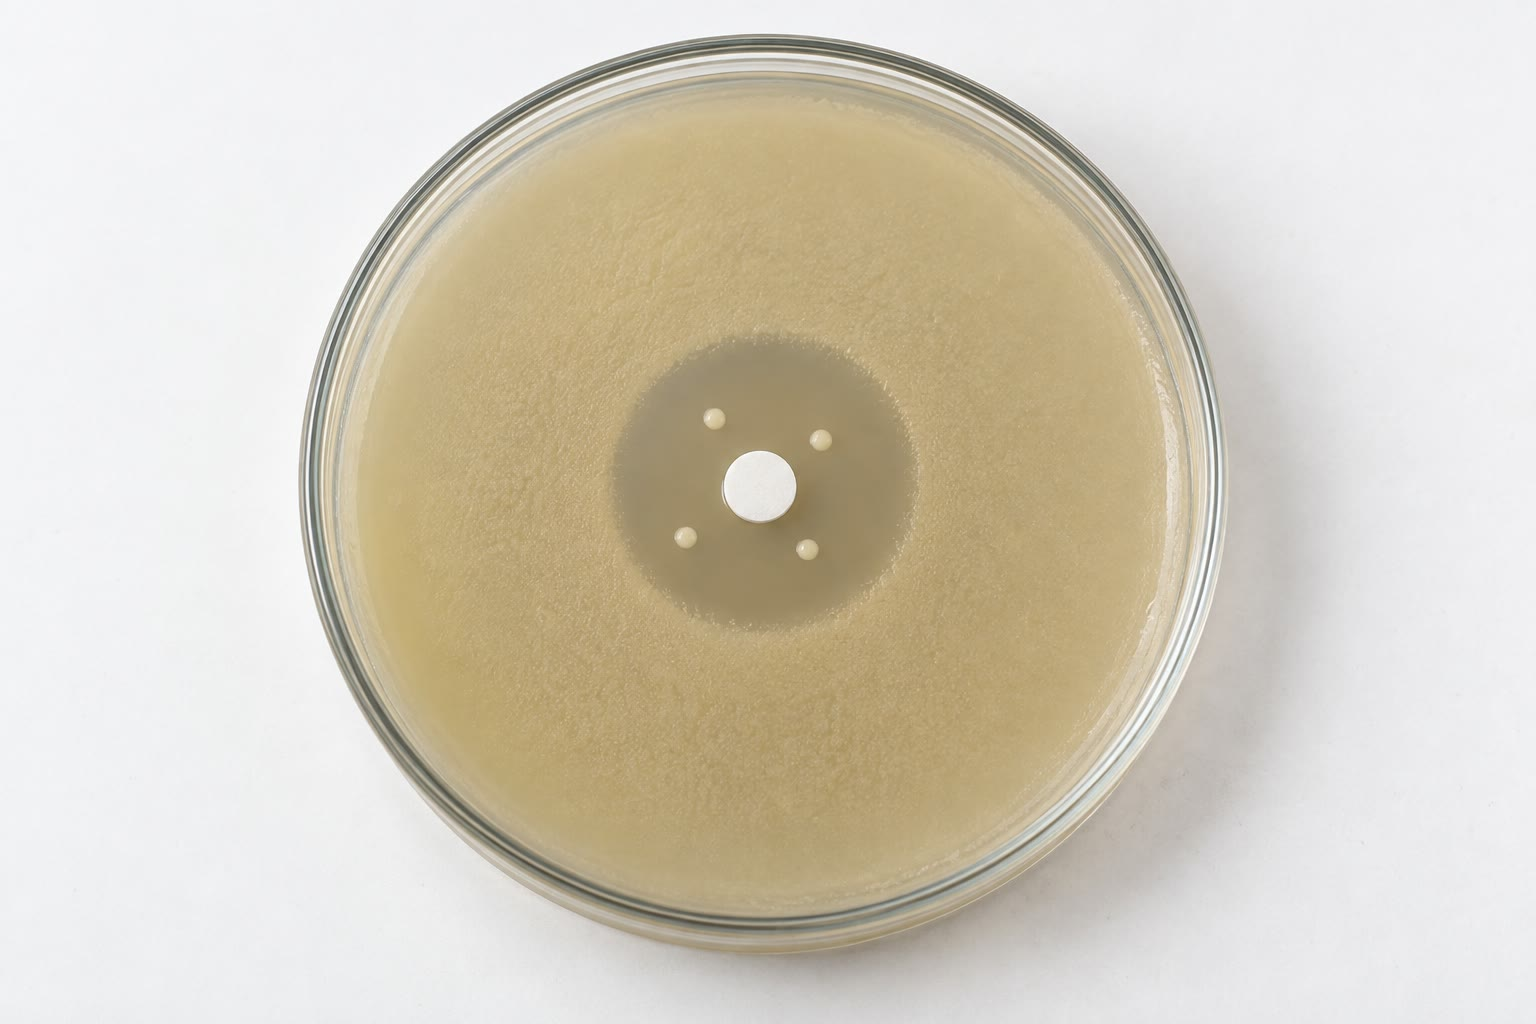
\includegraphics[width=0.5\linewidth]{images/book4/ai/b4-03-luria-plate.jpg}

{\small 细菌菌苔上的一张抗生素纸片：透明圈是
纸片扩散出的药物杀死敏感细胞的区域，圈内的
菌落则由放置纸片之前就已存在的
抗性\omterm{def:b2:genome-diversification:mutation}{突变}体长成。}
\end{omfigure}

\begin{proposition}[修复及其局限]\label{prop:b2:genome-diversification:repair}
\index{DNA 修复}
细胞在损伤成为\omterm{def:b2:genome-diversification:mutation}{突变}之前，会修正其中的大多数。
\emph{错配修复}清除新合成链上错误的碱基。
\emph{碱基切除修复}切除单个受损碱基（如尿嘧啶、
氧化的鸟嘌呤）并填补缺口；这正是 DNA 使用胸腺嘧啶
而非尿嘧啶的原因：DNA 中的尿嘧啶只能来自脱氨的胞嘧啶，
会被识别为外来物。\emph{核苷酸切除修复}切除
大体积损伤（如胸腺嘧啶二聚体）两侧约十二个碱基的一段序列；
缺乏该修复系统的人（着色性干皮病患者）在
普通日光照射下会患皮肤癌。
\emph{重组修复}则利用姐妹拷贝重建断裂的染色体。
逃过修复、或被错误修复的损伤即为\omterm{def:b2:genome-diversification:mutation}{突变}——
失去修复系统的细胞（即\emph{\omterm{def:b2:genome-diversification:mutation}{突变}子}）\omterm{thm:b2:genome-diversification:rate}{突变速率}快百倍，
这在压力下是短期优势，
但长期看则是负担。
修复机制将在本科三年级分册中深入讨论。
\end{proposition}

\section{会移动的基因}

\begin{definition}[转座元件]\label{def:b2:genome-diversification:transposon}
\index{转座子}\index{反转录转座子}
\emph{转座元件}是指可以在基因组中移动到新位置的
一段 DNA 序列。\emph{DNA 转座子}编码一种
\emph{转座酶}，它将该元件切下并插入他处
（或在那里复制一份）。细菌的插入序列是最简单的一类
（一个转座酶基因位于两个反向重复序列之间），
复合转座子则在两个插入序列之间携带额外的基因，
通常是抗生素抗性基因。\emph{反转录转座子}通过
一条以 RNA 为中间体的复制-粘贴途径移动，
RNA 再由逆转录酶拷贝回 DNA；它们从不离开原位，
因此不断积累。
落入某个基因中的元件会破坏该基因；
落在基因附近时，则可能改变其表达；
一条染色体上有两个拷贝时，会为不等交换提供位点。
转座子及其残迹占人类基因组的一半、玉米基因组的百分之八十；其中大多数如今已无法移动。
\end{definition}
\begin{proof}[证据]
麦克林托克（20 世纪 40 至 50 年代）研究了玉米籽粒，
其紫色色素在一些细胞中丢失、在另一些细胞中恢复，
从而形成斑点状籽粒。她通过杂交和染色体观察表明，
这种不稳定性是由一个元件（\emph{解离子}）引起的：
该元件在所处位置打断染色体，
并在第二个元件（\emph{激活子}）的控制下在不同位置之间移动；
当元件位于某基因中时，该基因被沉默，
当元件离开时，该基因又恢复活性。她由此得出结论：
基因可以改变位置。这一观点直到二十年后，
即在发现细菌插入序列之后，才被接受，
麦克林托克也因此于 1983 年获得诺贝尔奖。
\end{proof}

\begin{omfigure}
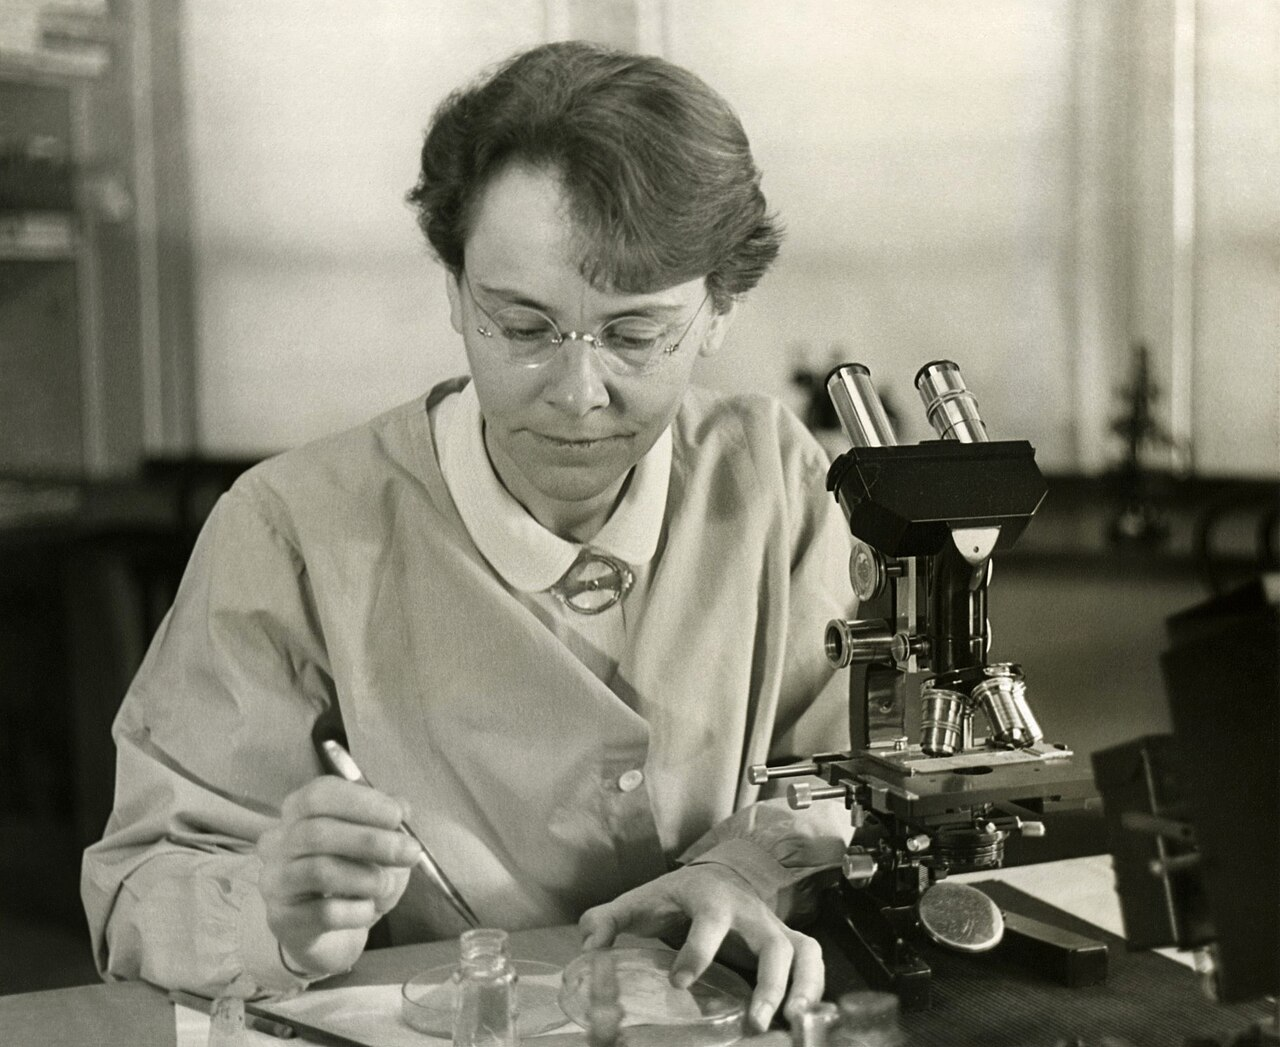
\includegraphics[width=0.4\linewidth]{images/book4/mcclintock.jpg}\hspace{0.04\linewidth}
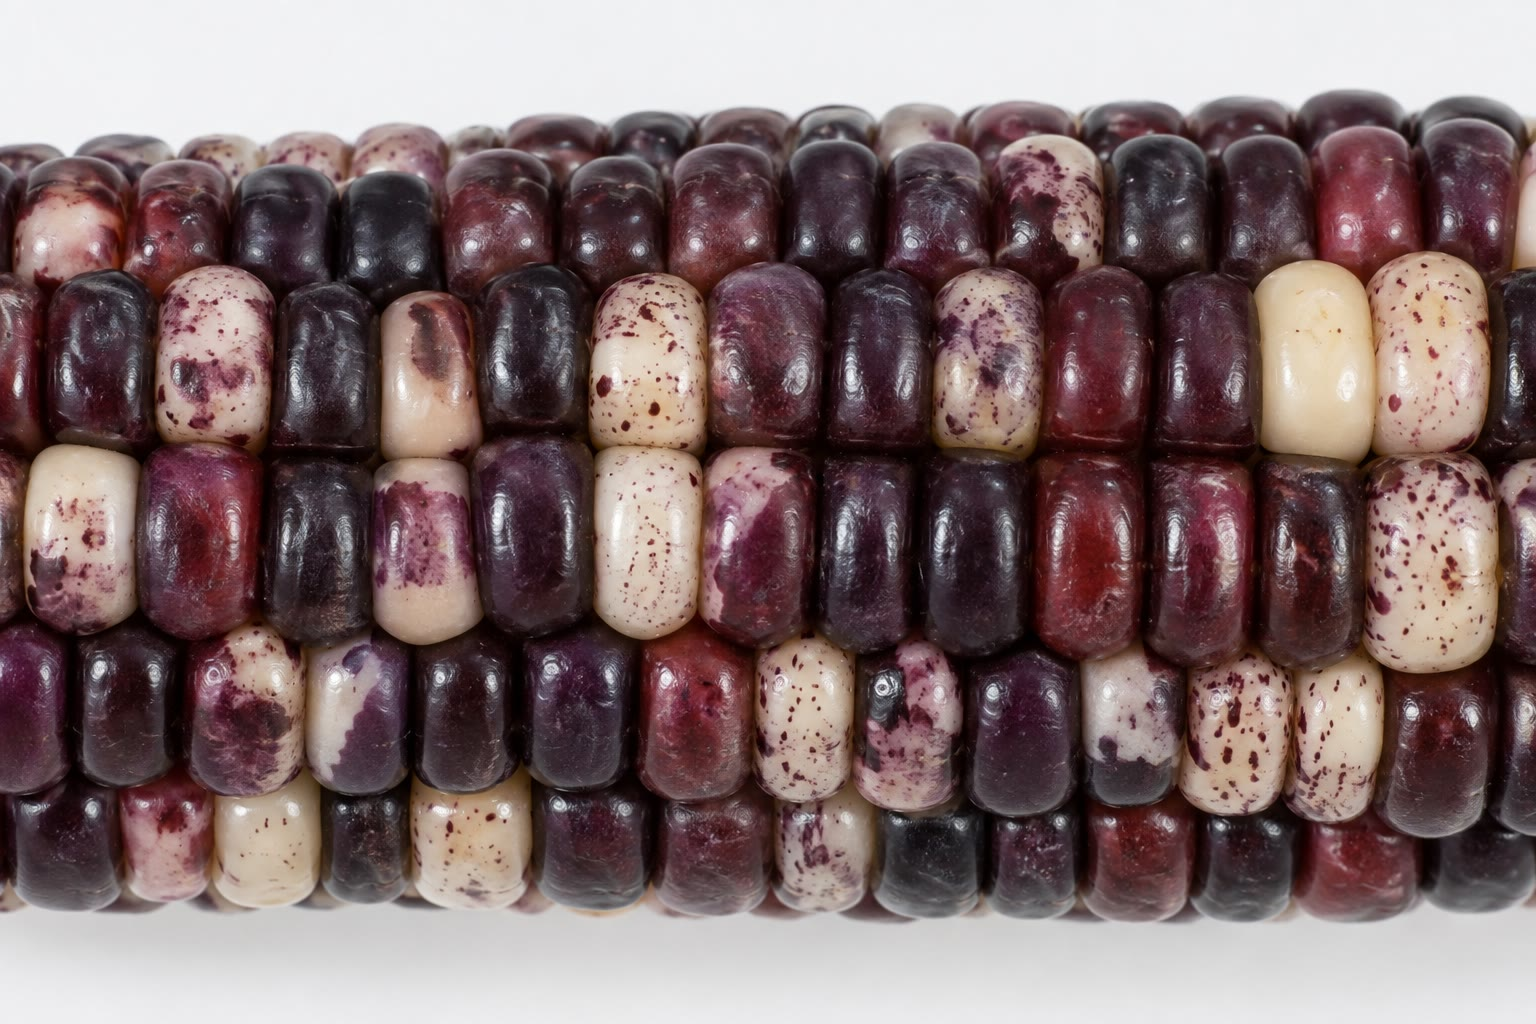
\includegraphics[width=0.5\linewidth]{images/book4/ai/b4-03-maize-kernels.jpg}

{\small 芭芭拉·麦克林托克，以及促使她发现转座元件的玉米籽粒：
一个紫色色素基因被插入的元件关闭，
当元件跳出时又在每个细胞中重新开启，
留下斑点和扇区。}
\end{omfigure}

\begin{omfigure}
\begin{tikzpicture}[every node/.style={font=\scriptsize}]
  % cut and paste
  \begin{scope}
    \draw[very thick, gray] (0,1.2) -- (4.5,1.2);
    \fill[omThm!70] (0.8,1.05) rectangle (1.8,1.35); \node[white, font=\tiny] at (1.3,1.2) {Tn};
    \draw[very thick, gray] (0,0) -- (4.5,0);
    \fill[omThm!70] (2.8,-0.15) rectangle (3.8,0.15); \node[white, font=\tiny] at (3.3,0) {Tn};
    \draw[->, thick, omThm] (1.3,1.0) .. controls (1.3,0.5) and (3.3,0.7) .. (3.3,0.2);
    \draw[dashed, gray] (0.8,1.2) -- (1.8,1.2);
    \node[align=center] at (2.25,-0.6) {剪切粘贴（DNA 转座子）：\\元件离开原位点};
  \end{scope}
  % copy and paste
  \begin{scope}[xshift=7.5cm]
    \draw[very thick, gray] (0,1.2) -- (4.5,1.2);
    \fill[omProp!80] (0.8,1.05) rectangle (1.8,1.35); \node[white, font=\tiny] at (1.3,1.2) {RT};
    \draw[very thick, gray] (0,0) -- (4.5,0);
    \fill[omProp!80] (2.8,-0.15) rectangle (3.8,0.15); \node[white, font=\tiny] at (3.3,0) {RT};
    \draw[->, thick, omProp] (1.3,1.0) .. controls (1.3,0.5) and (3.3,0.7) .. (3.3,0.2);
    \node[omProp, anchor=west, align=left] at (3.6,0.75) {RNA 拷贝，\\经逆转录};
    \node[align=center] at (2.25,-0.6) {复制粘贴（反转录转座子）：\\旧拷贝保留，拷贝数增加};
  \end{scope}
\end{tikzpicture}

{\small 两种移动方式。DNA \omterm{def:b2:genome-diversification:transposon}{转座子}被切除，
随后重新插入；\omterm{def:b2:genome-diversification:transposon}{反转录转座子}被转录，逆转录回 DNA，
并插入别处，因此其拷贝不断积累。}
\end{omfigure}

\begin{definition}[水平基因转移]\label{def:b2:genome-diversification:hgt}
\index{水平基因转移}\index{转化}\index{接合!细菌}\index{转导}
\omterm{def:b2:unicellular-diversity:prokaryote}{原核生物}通过三条途径从非亲代细胞获得基因。
\emph{转化}：细胞从周围环境摄取裸露 DNA
（由死亡细胞释放）并将其重组进自身染色体；
有些物种天然具有感受态，
肺炎链球菌正是借此途径交换荚膜基因。
\emph{接合}：携带接合性\omterm{def:b2:unicellular-diversity:prokaryote}{质粒}的供体
（\emph{E.~coli} 的 F 因子）形成菌毛，
将受体拉近，
并通过滚环复制，使\omterm{def:b2:unicellular-diversity:prokaryote}{质粒}的一条单链
经孔道转入受体；
若\omterm{def:b2:unicellular-diversity:prokaryote}{质粒}已整合进染色体（Hfr 菌株），
染色体基因便依次跟随其后被转移，
每个基因进入的时间即用于绘制染色体图谱。
\emph{转导}：噬菌体错误地包装了一段宿主 DNA，
并将其注入下一个被感染的细胞。
这些途径共同使耐药基因在医院内数年间在不同物种之间传播，
并且在地质时间尺度上将代谢基因传遍整个细菌谱系，
因此\omterm{def:b2:unicellular-diversity:prokaryote}{原核生物}的谱系与其说是一棵树，不如说是一张网（\cref{ch:b2:phylogenetic-trees}）。
\end{definition}
\begin{proof}[证据]
莱德伯格和塔特姆（1946）将两种 \emph{E.~coli} 菌株混合，
每种菌株都不能合成两种不同的营养物质，然后将混合物涂布于基本培养基上，
两者单独都无法生长：约每一千万个细胞中出现一个菌落，
能够合成全部四种物质——即重组体。
戴维斯（1950）重复了该实验，用滤膜将两种菌株隔开，
滤膜允许分子通过但不允许细胞通过，未出现重组体，因此需要细胞间接触。
随后海斯证明转移是单向的，即从供体到受体；
沃尔曼和雅各布（1956）
在搅拌器中每隔一段时间中断交配，发现供体的基因
以固定顺序、一个接一个地进入受体，
历时约一百分钟。
\end{proof}

\begin{omfigure}
\begin{minipage}[b]{0.56\linewidth}\centering
\begin{tikzpicture}[every node/.style={font=\scriptsize}]
  % donor
  \draw[thick, fill=omDef!8] (0,0) ellipse (1.5 and 0.75);
  \draw[thick, omDef] (0.2,0) circle (0.45);
  \draw[thick, omThm] (-0.9,0.1) circle (0.22);
  \node[anchor=south] at (0,1.25) {供体 $F^+$};
  \draw[omThm] (-0.9,-0.12) -- (-1.1,-1.0) node[below] {F 质粒};
  \draw[omDef] (0.4,-0.4) -- (0.6,-1.0) node[below] {染色体};
  % recipient
  \draw[thick, fill=omDef!8] (5,0) ellipse (1.5 and 0.75);
  \draw[thick, omDef] (5.2,0) circle (0.45);
  \node[anchor=south] at (5,1.25) {受体 $F^-$};
  % pilus
  \draw[very thick, omThm] (1.5,0) -- (3.5,0);
  \node[omThm, below] at (2.5,-0.05) {菌毛};
  % single strand transferred
  \draw[->, thick, omThm, dashed] (-0.7,0.15) .. controls (1.0,0.7) and (3.0,0.7) .. (4.1,0.4);
  \node[omThm, anchor=south] at (2.5,0.7) {单链经滚环复制};
  \draw[thick, omThm, dashed] (4.1,0.2) circle (0.2);
\end{tikzpicture}
\end{minipage}\hfill
\begin{minipage}[b]{0.42\linewidth}\centering
\begin{tikzpicture}
\begin{axis}[
  width=\linewidth, height=4.6cm,
  axis x line=bottom, axis y line=left,
  xmin=0, xmax=40, ymin=0, ymax=1.1,
  xlabel={中断搅拌前的分钟数}, ylabel={重组体（相对值）},
  xlabel style={font=\scriptsize, at={(axis description cs:0.5,-0.18)}, anchor=north},
  ylabel style={font=\scriptsize},
  tick label style={font=\scriptsize}, xtick={0,10,20,30,40}, ytick={0,0.5,1},
  legend style={font=\scriptsize, at={(0.97,0.08)}, anchor=south east, draw=none},
  clip=false,
]
\addplot[very thick, omDef, domain=8:40, samples=40] {1-exp(-(x-8)/5)};
\addlegendentry{\emph{thr}，\qty{8}{min}时进入}
\addplot[very thick, omProp, domain=17:40, samples=40] {1-exp(-(x-17)/5)};
\addlegendentry{\emph{lac} 基因，\qty{17}{min}}
\addplot[very thick, omThm, domain=25:40, samples=40] {1-exp(-(x-25)/5)};
\addlegendentry{\emph{gal} 基因，\qty{25}{min}}
\end{axis}
\end{tikzpicture}
\end{minipage}

{\small 左：接合——供体在复制的同时，经菌毛连接处传递其 F
\omterm{def:b2:unicellular-diversity:prokaryote}{质粒}的一条链。右：以 Hfr 供体进行的中断交配实验：染色体
上每个基因开始在重组体中出现的时刻各有特征，
各基因出现的时刻因此得以确定，
即以分钟为单位对染色体作图。}
\end{omfigure}

\begin{omfigure}
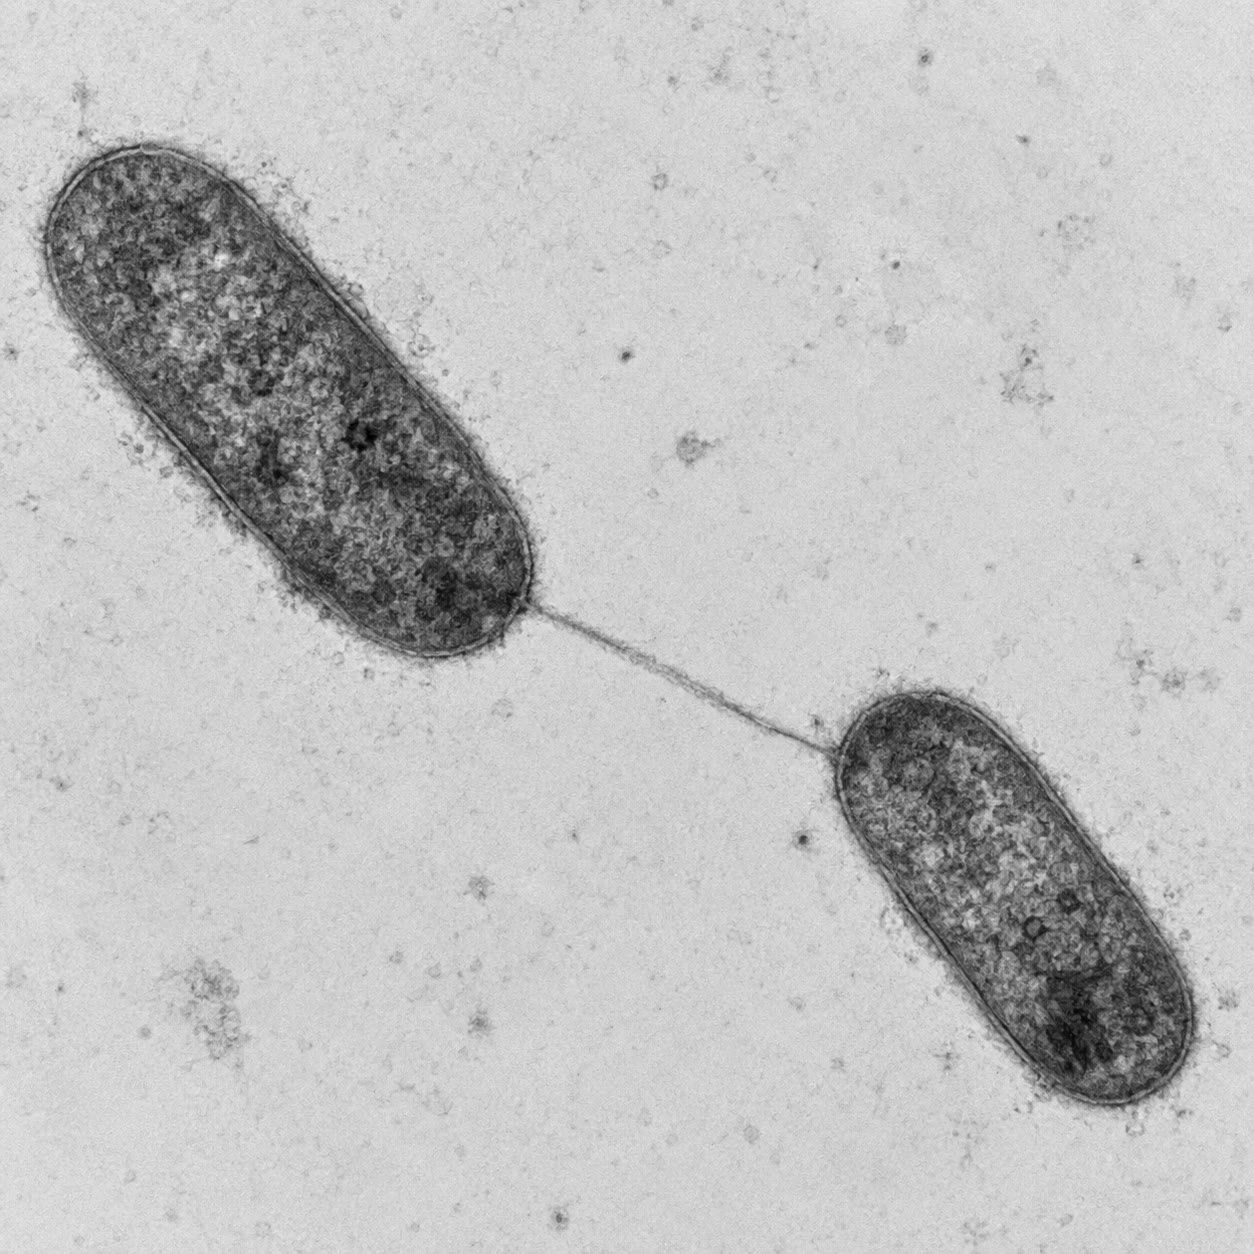
\includegraphics[width=0.42\linewidth]{images/book4/ai/b4-03-conjugation-tem.jpg}

{\small 两个细菌由接合性菌毛相连，经透射电子显微镜观察：
图中所示为\omterm{def:b2:unicellular-diversity:prokaryote}{质粒}借以转移的桥梁，
\omterm{def:b2:unicellular-diversity:prokaryote}{质粒}正是经此通过。}
\end{omfigure}

\begin{example}[耐药性的迁移]\label{ex:b2:genome-diversification:resistance}
耐药基因通常只起源一次：或由\omterm{def:b2:genome-diversification:mutation}{突变}产生，或来自
产生该抗生素的土壤细菌，随后便会迁移：先由染色体
转移到\omterm{def:b2:genome-diversification:transposon}{转座子}上，再从\omterm{def:b2:genome-diversification:transposon}{转座子}转移到接合性\omterm{def:b2:unicellular-diversity:prokaryote}{质粒}上，
再经接合作用跨物种转移，
经\omterm{def:b2:genome-diversification:hgt}{转导}作用跨菌株转移，并经
转化作用重新整合进染色体。同时携带五种或六种耐药性的\omterm{def:b2:unicellular-diversity:prokaryote}{质粒}
（在\emph{整合子}中组装，整合子可捕获基因盒）于
1950 年代在日本被发现，距药物投入使用仅数年。
其编码碳青霉烯酶 NDM-1 的基因，
首次发现于 2008 年，三年之内便借\omterm{def:b2:unicellular-diversity:prokaryote}{质粒}传遍每一大洲。
耐药性的演化主要不在于产生新基因，
而在于旧基因的迁移。
\end{example}

\section{重复：基因与基因组}

\begin{proposition}[基因重复与基因家族]\label{prop:b2:genome-diversification:duplication}
\index{基因重复}\index{基因家族}\index{不等交叉互换}
若染色体上两段相似序列串联排列，
同源染色体可能在减数分裂时错位配对，
并发生不等交换，使一条产物带三个拷贝，
另一条只带一个。重复基因是冗余的：一个拷贝可保留原有功能，
另一个拷贝则可自由积累\omterm{def:b2:genome-diversification:mutation}{突变}，通常退化为
\emph{假基因}，偶尔获得新功能，
（\emph{新功能化}）或分担旧功能
（\emph{亚功能化}）。经过数亿年，
这种重复便形成了\emph{\omterm{prop:b2:genome-diversification:duplication}{基因家族}}：珠蛋白（单个祖先基因
演化为肌红蛋白、$\alpha$ 簇和
$\beta$ 簇，胚胎型、胎儿型和成体型成员依次表达，
嗅觉受体（小鼠中有一千个基因），
同源框基因和晶状体蛋白。基因组中的大多数基因都属于一个
\omterm{prop:b2:genome-diversification:duplication}{基因家族}，重复是新基因的主要
来源。
\end{proposition}
\begin{proof}[证据]
人类 $\beta$-珠蛋白簇位于第 11 号染色体上，含有五个功能基因
（$\varepsilon$、$^{G}\gamma$、$^{A}\gamma$、
$\delta$、$\beta$），以及一个假基因，按发育中开启的先后排列，
它们都具有相同的外显子–内含子结构，分化时间
越近的，序列越相似；
第 16 号染色体上的 $\alpha$ 簇结构相同。
一个或多个 $\alpha$ 基因的缺失很常见，
它们由近乎相同的拷贝之间的不等交换产生，
并导致 $\alpha$-地中海贫血；其互补产物，
即带有三个 $\alpha$ 基因的染色体，
在同一人群中也可见到。
\end{proof}

\begin{omfigure}
\begin{tikzpicture}[every node/.style={font=\scriptsize}]
  % unequal crossing over
  \begin{scope}
    \draw[very thick, gray] (0,1.2) -- (5,1.2);
    \fill[omDef!70] (1.0,1.05) rectangle (2.0,1.35); \fill[omDef!70] (2.4,1.05) rectangle (3.4,1.35);
    \draw[very thick, gray] (0,0) -- (5,0);
    \fill[omDef!70] (1.0,-0.15) rectangle (2.0,0.15); \fill[omDef!70] (2.4,-0.15) rectangle (3.4,0.15);
    \node[above] at (1.5,1.35) {A}; \node[above] at (2.9,1.35) {A$'$};
    \draw[very thick, omThm] (2.9,1.05) -- (1.5,0.15);
    \node[align=center] at (2.5,-0.6) {错配的同源染色体 \\发生不等交换};
    \draw[->, thick, gray] (5.3,0.6) -- (6.1,0.6);
    % products
    \draw[very thick, gray] (6.5,1.2) -- (11.5,1.2);
    \fill[omDef!70] (7.5,1.05) rectangle (8.5,1.35); \fill[omDef!70] (8.9,1.05) rectangle (9.9,1.35); \fill[omDef!70] (10.3,1.05) rectangle (11.3,1.35);
    \node[above] at (9.4,1.35) {三个拷贝};
    \draw[very thick, gray] (6.5,0) -- (11.5,0);
    \fill[omDef!70] (7.5,-0.15) rectangle (8.5,0.15);
    \node[above] at (8.0,0.15) {一个拷贝};
  \end{scope}
  % globin family tree
  \begin{scope}[yshift=-3.6cm]
    \draw[thick] (2,2.2) -- (2,1.7);
    \draw[thick] (0.5,1.7) -- (3.5,1.7);
    \draw[thick] (0.5,1.7) -- (0.5,0.4); \node[below] at (0.5,0.4) {肌红蛋白};
    \draw[thick] (3.5,1.7) -- (3.5,1.2);
    \draw[thick] (2.3,1.2) -- (4.7,1.2);
    \draw[thick] (2.3,1.2) -- (2.3,0.4); \node[below] at (2.3,0.4) {$\alpha$ 家族};
    \draw[thick] (4.7,1.2) -- (4.7,0.9);
    \draw[thick] (3.6,0.9) -- (5.8,0.9);
    \draw[thick] (3.6,0.9) -- (3.6,0.4); \node[below] at (3.6,0.4) {$\varepsilon,\gamma$};
    \draw[thick] (5.8,0.9) -- (5.8,0.7);
    \draw[thick] (5.2,0.7) -- (6.4,0.7);
    \draw[thick] (5.2,0.7) -- (5.2,0.4); \node[below] at (5.2,0.4) {$\delta$};
    \draw[thick] (6.4,0.7) -- (6.4,0.4); \node[below] at (6.4,0.4) {$\beta$};
    \node[anchor=west, align=left] at (7.2,1.7) {一个祖先珠蛋白基因的重复：\\在脊椎动物出现之前（肌红蛋白/血红蛋白），\\约 4.5 亿年前（$\alpha$/$\beta$），\\随后在 $\beta$ 簇内部（胚胎型、胎儿型、成体型）};
    \node[anchor=east, gray] at (1.9,2.1) {祖先珠蛋白基因};
  \end{scope}
\end{tikzpicture}

{\small 上图：错配的串联拷贝之间发生不等交换，
产生一条带三个拷贝的染色体和一条只带一个拷贝的染色体。
下图：球蛋白家族，由相继的重复与
分化逐步形成。}
\end{omfigure}

\begin{definition}[多倍性]\label{def:b2:genome-diversification:polyploidy}
\index{多倍性}\index{异源多倍体}\index{同源多倍体}
具有两套以上完整染色体组的个体称为\emph{多倍体}。
\emph{同源多倍体}含有来自同一物种的若干套染色体组（减数分裂失败
产生二倍体配子，两个此类配子结合形成四倍体）；
\emph{异源多倍体}则合并两个物种的染色体组，
形成于杂交之后。二倍体杂种 AB 的任何染色体都没有同源染色体，
因而在减数分裂时无法配对，杂种不育；若其
基因组加倍为 AABB，每条染色体再次有了配对伙伴，减数分裂
得以正常进行，新植株可育，但无法与任一亲本回交
（其后代 AAB 不育）。多倍性因此可在一步之内形成
新物种，被子植物物种中约三分之一
是以此方式形成的：面包小麦为三种禾本科植物的六倍体 AABBDD，
园艺草莓为八倍体，棉花和烟草为异源四倍体，
脊椎动物谱系本身在其起源附近曾两次加倍基因组。
多倍体通常比
其二倍体祖先更大（DNA 更多，细胞更大），并
深受育种者青睐。
\end{definition}

\begin{omfigure}
\begin{tikzpicture}[every node/.style={font=\scriptsize}]
  \node[draw, rounded corners, fill=omDef!10, align=center] (a) at (0,0) {\emph{乌拉尔图小麦}\\AA, $2n = 14$};
  \node[draw, rounded corners, fill=omDef!10, align=center] (b) at (3.4,0) {\emph{山羊草}\\BB, $2n = 14$};
  \node[draw, rounded corners, fill=omProp!15, align=center] (ab) at (1.7,-1.5) {杂种 AB\\$n = 14$，不育};
  \node[draw, rounded corners, fill=omExo!25, align=center] (aabb) at (1.7,-3.1) {二粒小麦 AABB\\$2n = 28$，可育};
  \node[draw, rounded corners, fill=omDef!10, align=center] (d) at (6.4,-3.1) {\emph{节节麦}\\DD, $2n = 14$};
  \node[draw, rounded corners, fill=omProp!15, align=center] (abd) at (4.0,-4.6) {杂种 ABD\\$3n = 21$，不育};
  \node[draw, rounded corners, fill=omExo!25, align=center] (abd2) at (4.0,-6.1) {面包小麦 AABBDD\\$2n = 42$，可育};
  \draw[->, thick] (a) -- (ab); \draw[->, thick] (b) -- (ab);
  \draw[->, thick] (ab) -- (aabb) node[midway, right] {基因组加倍};
  \draw[->, thick] (aabb) -- (abd); \draw[->, thick] (d) -- (abd);
  \draw[->, thick] (abd) -- (abd2) node[midway, right] {基因组加倍};
  \node[anchor=west, align=left, gray] at (7.8,-1.5) {每次杂交产生的不育植株，\\染色体无法配对；\\每次加倍恢复配对与可育性——\\并形成 \\一个无法回交的物种};
\end{tikzpicture}

{\small 面包小麦的起源：两次杂交，每次之后都
接一次基因组加倍，由三种二倍体禾本科植物
在约一万年间形成了六倍体。}
\end{omfigure}

\begin{omfigure}
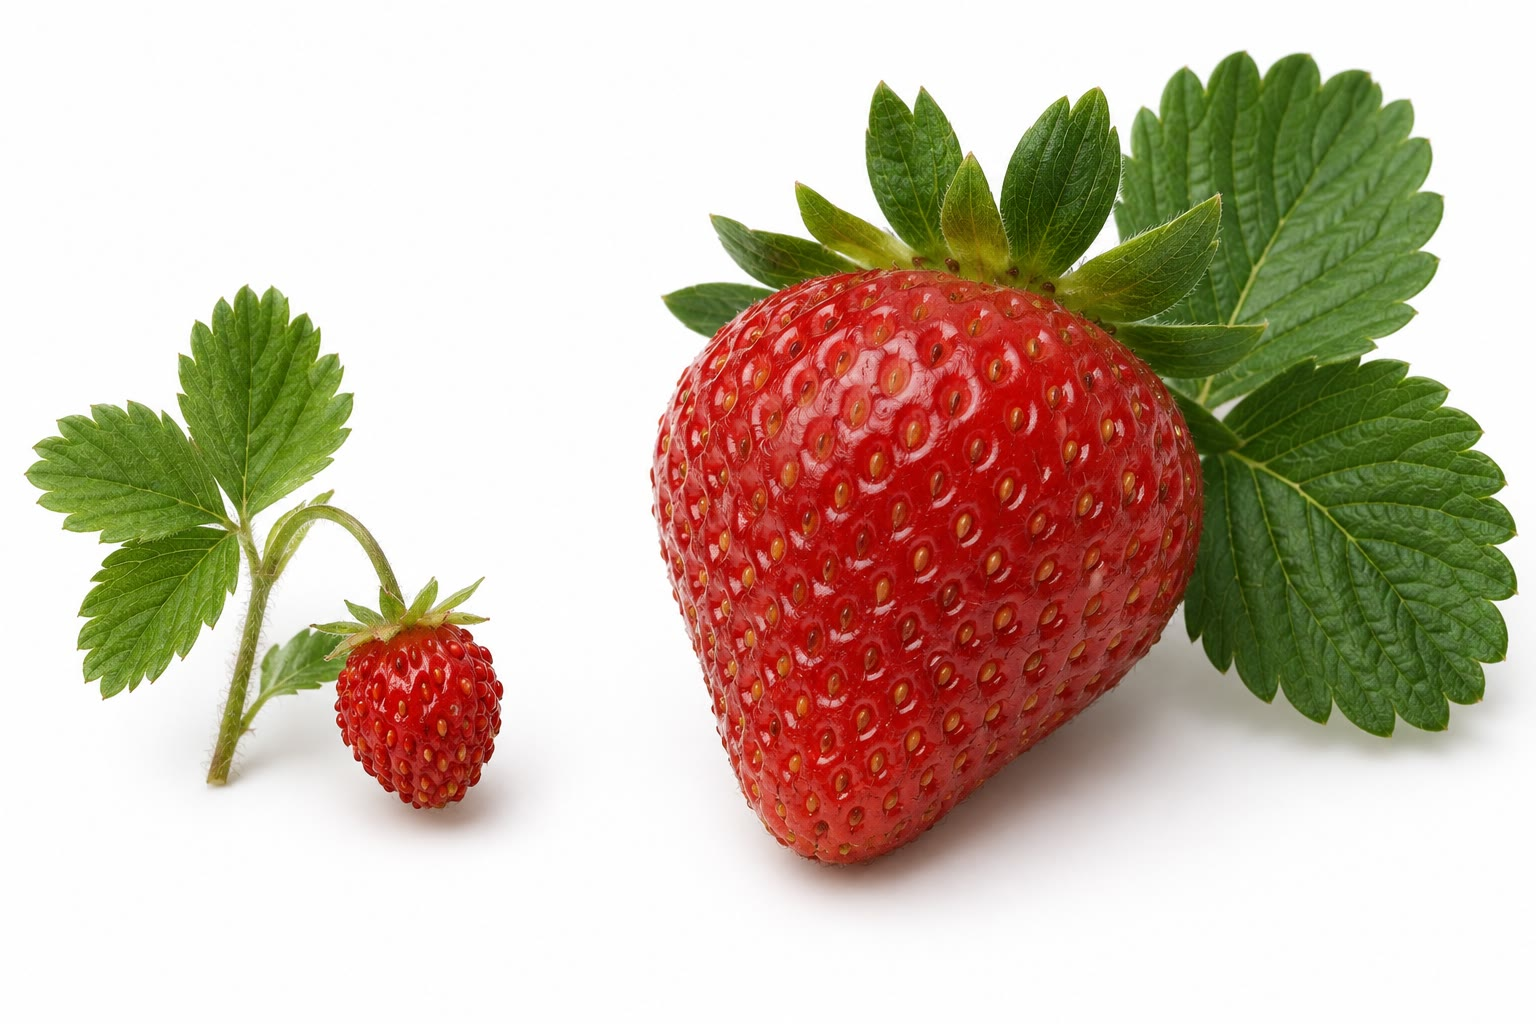
\includegraphics[width=0.55\linewidth]{images/book4/ai/b4-03-polyploid-strawberries.jpg}

{\small 野生二倍体草莓与栽培八倍体草莓：
\omterm{def:b2:genome-diversification:polyploidy}{多倍体}每个细胞的 DNA 为四倍，是
个体更大、果实也更大的植株。}
\end{omfigure}

\section{随机性与速率}

\begin{proposition}[突变相对于需要是随机的]\label{prop:b2:genome-diversification:random}
\index{突变!随机性}
\omterm{thm:b2:genome-diversification:luria}{波动试验}与影印培养表明，在新环境中有用的\omterm{def:b2:genome-diversification:mutation}{突变}
无论该环境是否存在，都以相同速率产生：
环境只是在\omterm{def:b2:genome-diversification:mutation}{突变}中进行选择，
而不是诱发\omterm{def:b2:genome-diversification:mutation}{突变}。\omterm{def:b2:genome-diversification:mutation}{突变}并非在所有意义上都是随机的：
转换多于颠换，CpG 二核苷酸
的\omterm{thm:b2:genome-diversification:rate}{突变速率}是其他位点的十倍（其
甲基化胞嘧啶\omterm{prop:b2:genome-diversification:sources}{脱氨基}为胸腺嘧啶，修复系统不能识别它
为外来物质），某些区域为热点，应激可
提高总体速率——但\omterm{def:b2:genome-diversification:mutation}{突变}对后果是盲目的。
\omterm{def:b2:genome-diversification:mutation}{突变}率本身是可遗传性状，选择会对其进行调节：
过高时，每一代都会遗传有害变化；过低时，
种群便无法跟上变化的世界。高\omterm{def:b2:genome-diversification:mutation}{突变}率菌株
在医院中短暂占优、长期则落败，而多数细胞
所维持的每碱基 $10^{-9}$ 速率，是在
错误成本与校对成本之间的折中。
\end{proposition}

\section{练习}

\begin{exercise}[$\star$]\label{exo:b2:genome-diversification:1}
对密码子 GAA（谷氨酸）的每一种改变进行分类：GAG；GTA；TAA；
在第一个碱基之后插入一个 C。哪些是转换，哪些是
颠换？
\end{exercise}

\begin{exercise}[$\star$]\label{exo:b2:genome-diversification:2}
已知每碱基对每次复制的\omterm{def:b2:genome-diversification:mutation}{突变}率为 $u = \qty{5e-10}{}$，基因组大小 $G =
\qty{4.6e6}{}$，一个 \emph{E.~coli} 细胞分裂一次平均产生
多少个新\omterm{def:b2:genome-diversification:mutation}{突变}？另外，在含有
$10^{9}$ 个细胞的培养物中每代产生多少个？
\end{exercise}

\begin{exercise}[$\star$]\label{exo:b2:genome-diversification:3}
列出基因水平转移的三种途径，并说明每种途径
需要什么（接触、病毒、游离 DNA），并说明通常
转移什么。
\end{exercise}

\begin{exercise}[$\star$]\label{exo:b2:genome-diversification:4}
区分同源\omterm{def:b2:genome-diversification:polyploidy}{多倍性}与异源\omterm{def:b2:genome-diversification:polyploidy}{多倍性}，各举一例，
并说明为什么两个物种的二倍体杂种通常
不育。
\end{exercise}

\begin{exercise}[$\star\star$]\label{exo:b2:genome-diversification:5}
人类生殖系每代每碱基对积累 $u = \qty{1.2e-8}{}$ 个\omterm{def:b2:genome-diversification:mutation}{突变}，
单倍体基因组长 \qty{3.2e9}{} 个碱基
对。一个孩子携带多少个新\omterm{def:b2:genome-diversification:mutation}{突变}？若 \qty{1.5}{\%}
的基因组编码蛋白质，编码区的 \qty{70}{\%}
替换会改变氨基酸，该孩子携带多少个新的
氨基酸改变？
\end{exercise}

\begin{exercise}[$\star\star$]\label{exo:b2:genome-diversification:6}
一个培养物从 $10^{3}$ 个细胞生长到 $10^{9}$ 个细胞；某一特定\omterm{def:b2:genome-diversification:mutation}{突变}
每次分裂中发生的概率为 $m = \qty{2e-8}{}$。计算
\omterm{def:b2:genome-diversification:mutation}{突变}事件数与\omterm{def:b2:genome-diversification:mutation}{突变}细胞数的期望值。为何不含\omterm{def:b2:genome-diversification:mutation}{突变}体的培养物所占比例
在此处无助于测量 $m$，而
需要多大的培养规模才能使其有用？
\end{exercise}

\begin{exercise}[$\star\star$]\label{exo:b2:genome-diversification:7}
胞嘧啶脱氨生成尿嘧啶；5-甲基胞嘧啶脱氨生成
胸腺嘧啶。说明前者为何能被高效修复，而后者不能，
并由此推断为何 CpG 位点（胞嘧啶在此被甲基化）
是\omterm{def:b2:genome-diversification:mutation}{突变}热点，且在基因组中出现的频率
低于随机情况下的预期。
\end{exercise}

\begin{exercise}[$\star\star$]\label{exo:b2:genome-diversification:8}
在中断接合实验中，四个基因进入受体细胞的时间分别为
8、17、25 和 \qty{40}{min}；整条染色体（\qty{4.6}{Mb}）
需要 \qty{100}{min}。将这些时间换算为
千碱基位置，并计算相邻基因之间的距离。
\end{exercise}

\begin{exercise}[$\star\star$]\label{exo:b2:genome-diversification:9}
画出配对与交叉互换过程，使两条各含两个串联
$\alpha$ 珠蛋白基因的染色体，变为一条含三个、一条含一个基因的染色体。
一人分别从父母各继承一条只含一个基因的染色体，
此人共有几个 $\alpha$ 基因，
其血红蛋白预期如何？
\end{exercise}

\begin{exercise}[$\star\star\star$]\label{exo:b2:genome-diversification:10}
普通小麦为 AABBDD 型，$2n = 42$。给出其配子的染色体数，
其起源各步中不育杂种的染色体数，以及
普通小麦与二粒小麦（AABB）杂交所得后代的染色体数。试从减数分裂配对的角度说明
为何每次染色体加倍都能恢复可育性，以及为何
六倍体无法与其亲本回交。
\end{exercise}

\begin{exercise}[$\star\star\star$]\label{exo:b2:genome-diversification:11}
在含 $N = 10^{9}$ 个细菌的肠道种群中，抗性\omterm{def:b2:unicellular-diversity:prokaryote}{质粒}
通过接合传播，传播速率与
携带者 $R$ 与非携带者 $N - R$ 的接触次数成正比：$\mathrm{d}R/\mathrm{d}t =
\gamma R (N - R)$，其中 $\gamma N = \qty{0.5}{h^{-1}}$。求解该方程，从一个携带者开始，
并计算种群中一半细菌携带该\omterm{def:b2:unicellular-diversity:prokaryote}{质粒}所需的时间。
若随后撤去抗生素，而该\omterm{def:b2:unicellular-diversity:prokaryote}{质粒}使宿主的生长速率
下降 \qty{5}{\%}，会发生什么？
\end{exercise}

\begin{exercise}[$\star\star\star$]\label{exo:b2:genome-diversification:12}
“\omterm{def:b2:genome-diversification:mutation}{突变}是随机的，而演化不是。”试结合\omterm{thm:b2:genome-diversification:luria}{波动试验}、影印平板法，
以及\omterm{def:b2:genome-diversification:mutation}{突变}率本身受选择这一事实，
进行讨论。
\end{exercise}

\section{问题：波动试验}

\begin{problem}[{周末问题——进行并分析一次波动试验，
由其中提取某一菌株的突变率，并将其换算到该菌株的基因组与种群规模，
模拟抗性质粒的扩散，
权衡突变体的代价，最后落脚于该菌株的
每碱基突变率与质粒取代种群所需的时间}]
\label{pb:b2:genome-diversification:1}
\emph{E.~coli} 培养物二十份，每份均从 \num{100}
个细胞开始，在 \qty{0.2}{mL} 中培养至 $N = \qty{2e8}{}$ 个细胞；每份
随后涂布于含噬菌体的平板上，并计数其中的抗性
菌落数：0, 0, 0, 1, 0, 0, 3, 0, 0, 1, 0, 0, 0, 0, 107,
0, 2, 0, 0, 5。与此同时，从同一大培养物中取二十份 \qty{0.2}{mL} 样品，
使其密度与上述相同，并同样涂板：
14, 15, 13, 21, 15, 14, 26, 16, 20, 13, 17, 12, 18, 14, 16, 19, 15,
13, 17, 16。基因组为 \qty{4.6e6}{} 碱基对，其中 \qty{88}{\%} 为编码序列。
对该噬菌体的抗性，可由某一受体基因中 \num{20} 种不同的
单碱基改变中任何一种引起。

\medskip
\noindent\textbf{第一部分——\omterm{thm:b2:genome-diversification:luria}{波动试验}。}
\begin{enumerate}
  \item 计算二十个独立培养物
        的均值与方差。
  \item 计算二十份样品的均值与方差。
  \item 对泊松分布而言，方差等于均值。
        哪一组服从泊松分布，各组的分布分别说明
        \omterm{def:b2:genome-diversification:mutation}{突变}\emph{何时}发生？
  \item 解释计数为 107 的原因。
  \item 独立培养物中有多少份不含\omterm{def:b2:genome-diversification:mutation}{突变}体？利用
        $p_0 = e^{-m(N - N_0)}$ 估计 $m$，即每次细胞分裂
        中\omterm{def:b2:genome-diversification:mutation}{突变}为抗性的速率。
  \item 计算每份培养物中\omterm{def:b2:genome-diversification:mutation}{突变}体细胞的期望数，所用公式为
        $mN\ln(N/N_0)$，并与观测均值相比较。
  \item 为何来自同一大培养物的样品，
        对 $m$ 的估计通过 $p_0$ 方法毫无用处？
\end{enumerate}

\medskip
\noindent\textbf{第二部分——换算到基因组。}
\begin{enumerate}[resume]
  \item 推算每个碱基对、每次复制的\omterm{def:b2:genome-diversification:mutation}{突变}率 $u$，
        由 $m$ 及赋予抗性的改变数目求得。
  \item 计算每个基因组每次复制产生的新\omterm{def:b2:genome-diversification:mutation}{突变}
        的平均数目 $U$。
  \item 一升培养物，细胞密度为 $10^{9}$ 个每毫升，
        倍增一次，种群中会出现多少个新\omterm{def:b2:genome-diversification:mutation}{突变}？
  \item 该基因组中可能出现的不同单碱基改变有多少种？
        平均而言，每一种改变在这一次倍增中
        出现多少次？
  \item 解释为何在这样的种群中，对任何一种单次\omterm{def:b2:genome-diversification:mutation}{突变}即可克服的
        单一抗生素，抗性实际上几乎
        必然存在。
  \item 解释联合使用两种抗生素（每种都需两次独立\omterm{def:b2:genome-diversification:mutation}{突变}）时，
        情况为何会改变？请用数字说明。
\end{enumerate}

\medskip
\noindent\textbf{第三部分——\omterm{def:b2:unicellular-diversity:prokaryote}{质粒}的扩散。}
在一个含 $N = 10^{9}$ 个细胞的肠道中，一个细胞获得了一个可接合的
抗性\omterm{def:b2:unicellular-diversity:prokaryote}{质粒}。携带者 $R$ 经接触将其传递：
$\mathrm{d}R/\mathrm{d}t = \gamma R(N - R)$，其中 $\gamma N =
\qty{0.5}{h^{-1}}$.
\begin{enumerate}[resume]
  \item 证明 $R(t) = N/\bigl(1 + (N - 1)e^{-\gamma N t}\bigr)$
        是满足 $R(0) = 1$ 的该方程的解。
  \item 计算一半细胞携带\omterm{def:b2:unicellular-diversity:prokaryote}{质粒}的时刻。
  \item 计算携带\omterm{def:b2:unicellular-diversity:prokaryote}{质粒}的细胞达到 \qty{99}{\%} 的时刻。
  \item 在半数细胞为携带者的时刻，每小时
        发生多少次接合事件？
  \item 将其与抗性\emph{\omterm{def:b2:genome-diversification:mutation}{突变}体}达到半数种群所需的时间相比较：
        该\omterm{def:b2:genome-diversification:mutation}{突变}体在抗生素作用下生长速率比其余细胞快 \qty{10}{\%}，
        敏感细胞的\omterm{def:b2:unicellular-diversity:division}{世代时间}为 \qty{1}{h}，
        从单个细胞出发，
        需要多长时间？
  \item 试总结为何抗性主要通过传递，而非通过
        后代繁衍而扩散。
\end{enumerate}

\medskip
\noindent\textbf{第四部分——增变株。}
缺乏错配修复的菌株，\omterm{def:b2:genome-diversification:mutation}{突变}速度快 \num{100} 倍。
设编码序列中 \qty{30}{\%} 的\omterm{def:b2:genome-diversification:mutation}{突变}有害。
\begin{enumerate}[resume]
  \item 计算该菌株的 $U$，以及每个细胞每代的
        有害\omterm{def:b2:genome-diversification:mutation}{突变}平均数目。
  \item 经过 \num{200} 代后，一个谱系的后代中，
        完全不携带有害\omterm{def:b2:genome-diversification:mutation}{突变}的比例为多少（按泊松分布计算）？
  \item 对野生型计算同样的量。
  \item 在上述\omterm{thm:b2:genome-diversification:luria}{波动试验}中，该增变株给出的平均计数会是多少，
        以及不含\omterm{def:b2:genome-diversification:mutation}{突变}体的培养物占多大比例，
        分别为多少？
  \item 用两句话解释，增变株为何常见于医院分离株，
        而在自然界中却较为罕见。
  \item 给出结果：该菌株的 $m$、$u$、$U$，以及
        \omterm{def:b2:unicellular-diversity:prokaryote}{质粒}在肠道中达到半数与 \qty{99}{\%} 所需的时间。
\end{enumerate}
\end{problem}
